\documentclass[final,11pt,a4paper]{article}
\usepackage[docversion = 0.0.1]{reportpackage}
%\setenumerate{label=\textbf{\arabic*}.}
\setlength{\baselineskip}{17pt}
\setmathrm{CMU Serif}[Scale=1.1]
\setlength{\parskip}{0.7em}
\renewcommand{\baselinestretch}{1.45}
\usepackage{cite}
\usepackage{tocloft}
\usepackage{cleveref}
\usepackage{url}
\usepackage{titlesec}
\setlength\cftparskip{-1.5pt}
\setlength\cftbeforesecskip{6pt}
\setcounter{tocdepth}{2}
\renewcommand{\figurename}{ภาพที่}
\renewcommand{\refname}{บรรณานุกรม}
\titlespacing\subsubsection{0pt}{0pt plus 4pt minus 2pt}{0pt plus 2pt minus 2pt}
\titlespacing\subsection{0pt}{0pt plus 4pt minus 2pt}{0pt plus 2pt minus 2pt}
\titlespacing\section{0pt}{0pt plus 4pt minus 2pt}{0pt plus 2pt minus 2pt}
\captionsetup[subfigure]{justification=justified,singlelinecheck=false}
\begin{document}
\section*{คำนำ}
รายงานฉบับนี้เป็นส่วนหนึ่งของรายวิชา 01026208 ELECTRICAL INSTRUMENTS AND MEASUREMENTS 
โดยมีจุดประสงค์เพื่อการศึกษาหลักการทำงาน ข้อได้เปรียบ และข้อจำกัดของอุปกรณ์วัดระดับที่ใช้ในอุตสาหกรรมประเภทต่างๆ 
เนื้อหาของรายงานฉบับนี้ จะเริ่มต้นด้วยการอธิบายถึงประเภทของการวัดระดับต่างๆ แล้วลงรายละเอียดเกี่ยวกับหลักการทำงานของอุปกรณ์วัดระดับในอุตสาหกรรมที่นิยมใช้
7 ชนิด ได้แก่ อุปกรณ์วัดระดับแบบลอย อุปกรณ์วัดระดับทางแสง สวิตช์ระดับแบบสภาพความนำ สวิตช์ระดับแบบสั่น อุปกรณ์วัดระดับแบบความจุไฟฟ้า 
อุปกรณ์วัดระดับระดับแบบใช้คลื่นเหนือเสียง (อัลตราโซนิค) และอุปกรณ์วัดระดับแบบเรดาร์

รายงานฉบับนี้เสร็จสมบูรณ์ได้ด้วยความอนุเคราะห์ช่วยเหลือจากผู้มีพระคุณหลายท่าน กลุ่มผู้จัดทำต้องขอขอบพระคุณ 
ผู้ช่วยศาสตราจารย์ ดร.นิรุธ จิรสุวรรณกุล ผู้ให้ความรู้และแนวทางการศึกษา และขอขอบคุณเพื่อน ๆ ทุกคนในคณะวิศวกรรมศาสตร์ สจล. ที่ให้ความช่วยเหลือมาโดยตลอด 
กลุ่มผู้จัดทำหวังว่ารายงานฉบับนี้จะให้ความรู้ แนวทางเกี่ยวกับการวัดระดับในอุตสาหกรรม ที่เป็นประโยชน์แก่ผู้สนใจทุกๆ ท่านบ้างไม่มากก็น้อย 

\vspace{1cm}
\hspace{9cm}
\vbox{\noindent
    นายปรัตถ์ คงไทย\\
    นายคณพศ ไชยมณีกร (บรรณาธิการ)\\
    นายญาณันธร เชิดชูไทย\\
    นายธนกฤต กิตติบรรพชา\\
    นางสาวนันท์นภัส แดงเรือง\\
    นายนิธิศ อรัญวาส\\
    นายริมทวีป กู่สุดใจ\\

}
\newpage
\renewcommand\contentsname{สารบัญ}
\tableofcontents
\newpage
\section{บทนำ}
การวัดระดับ (Level Measurement) คือการระบุตำแหน่งของพื้นผิวภายในถัง เครื่องปฏิกรณ์
หรือภาชนะอื่นๆ โดยวัดระยะห่างแนวตั้ง (Vertical Distance) ระหว่างจุดอ้างอิงซึ่งโดยปกติคือฐานของภาชนะ กับพื้นผิว
ของของเหลว ของแข็ง หรือส่วนต่อประสานของของเหลวสองชนิด

การวัดระดับมีความสำคัญต่ออุตสาหกรรมเป็นอย่างมาก เพราะการทราบระดับของวัตถุดิบ และผลิตภัณฑ์ในกระบวนการผลิตต่างๆ
ทำให้สามารถจัดการระบบการผลิตได้อย่างมีแม่นยำ มีประสิทธิภาพ ช่วยเพิ่มความสามารถในการแข่งขันขององค์การ 
และที่สำคัญคือช่วยให้กระบวนการผลิตมีความปลอดภัย ซึ่งปัจจัยสำคัญทำให้ผู้ผลิต ได้รับไว้วางใจจากกลุ่มลูกค้า ผู้ลงทุน และประชาชนโดยรอบสถานที่ผลิต
โดยความสำคัญของการวัดระดับต่ออุตสาหกรรมในมิติต่างๆ พอจะสรุปได้ดังนี้ 
\begin{enumerate}
    \item \textbf{ประสิทธิภาพของกระบวนการผลิต} การทราบปริมาณที่แน่นอนจากการวัดระดับที่แม่นยำ
    ช่วยเพิ่มประสิทธิภาพของกระบวนการผลิต ผู้ผลิตสามารถจัดสรรทรัพยากรที่มีได้อย่างมีประสิทธิภาพ 
    และลดค่าใช้จ่ายในการจัดซื้อและบำรุงรักษาถังเก็บที่ไม่จำเป็น
    \item \textbf{ความปลอดภัย} การวัดระดับมีบทบาทอย่างมากในการรักษาความปลอดภัยในอุตสาหกรรม
    ความล้มเหลวในระบบวัดระดับ จนทำให้เกิดการบรรจุเกินจนล้น อาจนำไปสู่หายนะ ทำให้สารอันตรายเกิดการรั่วไหล
    สร้างความเสียหายต่อชีวิตและทรัพย์สิน รวมทั้งสิ่งแวดล้อมโดยรอบอย่างมหาศาลได้ 
    \item \textbf{มูลค่าของสินค้า} บ่อยครั้งมูลค่าของสินค้าที่เป็นของเหลว หรือของแข็งในถังเก็บ
    ขึ้นอยู่กับน้ำหนัก หรือปริมาตรของสินค้า ซึ่งคำนวณได้จากระดับของสินค้านั้นๆ 
    ความคลาดเคลื่อนในการวัดระดับเพียง $1/8$ นิ้ว ($\approx 3$ มิลลิเมตร) 
    จึงอาจส่งผลต่อมูลค่าของสินค้าได้อย่างมหาศาล โดยปกติเครื่องวัดที่ใช้วัดระดับในการซื้อขาย
    โอนกรรมสิทธิ์ในสินค้าตามกฏหมายจะมีความคลาดเคลื่อนในการวัดระดับน้อยกว่า  $1/16$ นิ้ว ($\approx 1$ มิลลิเมตร)
    และได้รับการอนุมัติจากหน่วยงานทางมาตรวิทยา
\end{enumerate}
\newpage
\section{ประเภทของการวัดระดับ และข้อพิจารณาในการเลือกเครื่องวัดระดับ}
\subsection{ประเภทของการวัดระดับ}
\subsubsection{การวัดระดับแบบต่อเนื่อง และแบบจุด}
\textbf{การวัดระดับแบบต่อเนื่อง} (Continuous Level Measurement) ระบุระดับของของเหลวเหนือช่วงการวัด (Full Span of Measurement)
หนึ่ง ส่วน\textbf{การวัดระดับแบบจุด} (Point Level Measurement) เป็นการวัดระดับที่บอกได้แต่เพียงว่า ของเหลวที่ทำการวัดอยู่ ``เหนือ'' 
หรือ ``ใต้'' เครื่องวัดเท่านั้น ไม่สามารถบอกระดับของเหลวได้ ในอุตสาหกรรม เครื่องวัดระดับแบบต่อเนื่องถูกใช้เพื่อควบคุมกระบวนการ (Process Control)
รวมถึงควบคุมและจัดการสินค้าคงคลัง (Inventory Control and Management) ส่วนเครื่องวัดระดับแบบจุด จะถูกใช้ร่วมกับเครื่องวัดแบบต่อเนื่อง 
เพื่อให้สัญญาณเตือนในกรณีที่ระดับของเหลวในถังเก็บอยู่สูง หรือต่ำเกินไป
\subsubsection{การวัดระดับแบบสัมผัส และไม่สัมผัส}
ใน\textbf{การวัดระดับแบบสัมผัส} (Contacting Level Measurement) ส่วนใดส่วนหนึ่งของระบบการวัด จะมีการสัมผัสโดยตรงกับของเหลวในถังเก็บ
เช่น การวัดระดับโดยใช้เรดาร์แบบบังคับนำคลื่น และลูกลอยเป็นต้น ส่วนใน\textbf{การวัดระดับแบบไม่สัมผัส} (์Non-contacting Level Measurement)
จะไม่มีส่วนของระบบการวัด ที่สัมผัสกับของเหลวที่ต้องการวัดเลย การวัดลักษณะนี้มักถูกใช้วัดระดับของเหลวและของแข็งที่ไม่สามารถวัดแบบสัมผัสได้ เช่น
ของเหลวมีฤทธิ์กัดกร่อนสูง ของแข็งที่ระเหิดได้ ของเหลวความหนืดสูง หรือวัตถุที่สกปรกมาก เป็นต้น
\subsubsection{การวัดระดับแบบวัดโดยตรง และโดยอ้อม}
\textbf{การวัดระดับโดยตรง} (Direct Level Measurement) เป็นการวัดระดับของเหลวโดยไม่ผ่านตัวแปรอื่น ตัวอย่างเช่น
 การวัดระดับน้ำมันเครื่องในรถ ดัวยแท่งวัด (Dipstick) ที่ให้ค่าออกมาเป็นระดับของน้ำมันเครื่องในถังเก็บโดยตรง 
 ส่วน \textbf{การวัดระดับโดยอ้อม} (Indirect Level Measurement) เป็นเทคนิคการวัดระดับของของเหลวโดยผ่านตัวแปรอื่นที่มีความสัมพันธ์กับระดับ เช่น กระแสที่ไหลในวงจร 
 เวลาที่คลื่นใช้ในการเดินทาง และอื่นๆ จากนั้นแปลงค่าที่ได้เป็นระดับของของเหลวด้วยกระบวนการทางคณิตศาสตร์
\subsection{ข้อพิจารณาในการเลือกเครื่องมือวัดระดับ}
เครื่องมือวัดระดับมีหลายประเภท แต่ละประเภทก็จะมีหลักการทำงาน ข้อได้เปรียบและข้อจำกัดที่แตกต่างกันไป 
ดังนั้นการเลือกเครื่องมือวัดระดับให้ถูกต้องเหมาะสมกับการใช้งานจึงมีความสำคัญ และจำเป็นอย่างยิ่ง ข้อพิจารณาในการเลือกเครื่องมือวัดระดับเบื้องต้นมีดังนี้
\subsubsection{จุดประสงค์ของการวัดระดับ} 
การทราบจุดประสงค์ที่แท้จริงของการทำการวัดเป็นสิ่งที่สำคัญอย่างมาก เพราะจะทำให้ทราบถึงข้อมูลที่ต้องการจากเครื่องวัด และเลือกประเภทการวัดที่เหมาะสมได้
เช่นถ้าผู้ใช้ต้องการระบบป้องกันการล้น และทราบจุดที่ต้องทำการเติมถังเก็บ เครื่องวัดระดับแบบจุดก็อาจเพียงพอต่อการใช้งาน 
แต่ถ้าผู้ใช้ต้องการทราบระดับของของเหลวภายในช่วงหนึ่งของถังเก็บ ก็จำเป็นที่จะต้องใช้เครื่องวัดระดับแบบต่อเนื่อง
\subsubsection{เงื่อนไขภายในถังเก็บ}
เครื่องวัดระดับประเภทต่างๆ สามารถทนต่ออุณหภูมิ และความดันในถังเก็บได้ไม่เท่ากัน สำหรับเครื่องวัดบางประเภท ความแม่นยำของการวัดจะขึ้นกับอุณหภูมิภายในถังเก็บ
นอกจากนี้การคน ความปั่นป่วน และไอเหนือของเหลวสามารถทำให้ค่าที่วัดได้เกิดความคลาดเคลื่อนได้ 
\subsubsection{คุณลักษณะของของเหลวที่ทำการวัด}
คุณลักษณะของของเหลวอาจส่งผลต่อเครื่องวัดได้ในหลายรูปแบบ ของเหลวที่หนืดอาจอุดที่หัววัด ไอน้ำ ฟองหรือฝุ่นเหนือของเหลวอาจรบกวนสัญญาณที่ถูกส่งมา 
นอกจากนี้ ค่าคงตัวไดอิเล็กตริกของของเหลวอาจทำให้ค่าจากเครื่องวัดระดับแบบความจุไฟฟ้าเปลี่ยนแปลงไป
และของเหลวอาจเคลือบติดหัววัดส่งผลต่อความไว (Sensitivity) ของเครื่องวัดที่อาศัยการสัมผัส 
\subsubsection{ข้อพิจารณาอื่นๆ} นอกจากข้อพิจารณาที่สำคัญทั้งสามข้างต้นแล้ว ยังมีข้อพิจารณาในประเด็นอื่นๆ เช่น 
ความเที่ยงตรง (Accuracy) และต้นทุนรวม (Total Cost) ของเครื่องมือวัด รวมทั้งความยากง่ายในการติดตั้ง, ปรับเทียบ, บำรุงรักษา 
และการใช้งานประจำวัน เป็นต้น

\newpage
\section{หลักการทำงานของเครื่องวัดระดับในอุตสาหกรรม}
\subsection{อุปกรณ์วัดระดับแบบลอย (Float Level Device)}
\subsubsection{หลักการทำงาน} 
อุปกรณ์วัดระดับแบบลอย เป็นเครื่องวัดระดับที่มีหลักการทำงานง่ายที่สุดแบบหนึ่ง
โดยเครื่องวัดระดับแบบลอยอย่างง่าย จะประกอบด้วยลูกลอยที่เป็นวัสดุลอยน้ำทรงกลม (Spherical) ทรงกระบอก (Cylindrical)
หรือเป็นทรงรีคล้ายแคปซูลยา (Oblong) ที่ถูกติดอยู่กับก้านกลไก เมื่อนำวัสดุลอยน้ำนี้ไปลอยน้ำ การเคลื่อนที่ของก้านกลไกจะเป็นไปโดยสอดคล้องกับระดับน้ำ
และสามารถเป็นตัวบอกระดับบนแผ่นเกจ (Guage Board) หรือกระตุ้นสวิตช์สำหรับส่งสัญญาณ หรือใช้ควบคุมการปิด-เปิดของเครื่องสูบน้ำ (Pump) ให้ทำงานได้โดยอัตโนมัติได้  

\subsubsection{รูปแบบของอุปกรณ์วัดระดับแบบลอย}
หลักการของเครื่องวัดระดับแบบลอย อาจนำไปสร้างเป็นเครื่องวัดในอุตสาหกรรมได้หลากหลายรูปแบบ โดยแต่ละรูปแบบก็จะเหมาะกับสภาพแวดล้อม 
และการใช้งานที่ต่างกันไป รูปแบบหลักๆ ของเครื่องวัดระดับแบบลอยสรุปได้ดังนี้
\begin{enumerate}
    \item \textbf{สวิตช์ลอยแบบเชื่อมต่อด้วยแม่เหล็ก (Magnetic Coupled Float Switch)} สวิตช์ลอยชนิดนี้ใช้การเชื่อมต่อทางแม่เหล็ก (Magnetic Coupling)
    ข้ามท่อปิดเพื่อแยกระหว่างของเหลวในกระบวนการและอุปกรณ์สวิตช์ของเครื่องวัด โดยมีโครงสร้างภายในแสดงได้ดังภาพที่  \ref{fig:mcfs} (\subref{fig:mcfs1})
    เมื่อระดับของเหลวเพิ่มสูงขึ้น  แม่เหล็กที่ติดอยู่จะพลิกกลับลงมากระตุ้นสวิตช์ให้เกิดการเปลี่ยนสถานะไป นอกจากนี้ยังอาจใช้หรีดสวิตช์ (Reed Switch) ที่เป็นหน้าสัมผัสขนาดเล็กบรรจุอยู่ในหลอดแก้ว 
    ช่วยลดขนาดและจำนวนส่วนเคลื่อนที่ ดังภาพที่ \ref{fig:mcfs} (\subref{fig:mcfs2})
    \item \textbf{ลูกลอยและท่อนำ (Float and Guide Tube)} สวิตช์ลอยรูปแบบนี้ประกอบด้วยลูกลอยทรงกลมซึ่งถูกร้อยผ่านท่อนำที่ไม่ติดแม่เหล็ก
    แม่เหล็กรูปวงแหวนจะถูกฝังอยู่ในลูกลอย และหรีดสวิตช์จะถูกผนึกอยู่ในท่อนำดังภาพที่ \ref{fig:mcfs} (\subref{fig:mcfs3}) ในจุดที่ต้องการ เมื่อระดับของเหลวเพิ่มขึ้น ลูกลอยที่มีแม่เหล็กอยู่ภายใน
    จะลอยขึ้นตามท่อนำ โดยเมื่อลอยขึ้นถึงตำแหน่งที่ฝังหรีดสวิตช์ไว้ หรีดสวิตช์ก็จะเปลี่ยนสถานะไป
    \item \textbf{สวิตช์เอียง (Tilt Switch)} สวิตช์เอียงเป็นลูกลอยพลาสติกที่ภายในมีสวิตช์ปรอทบรรจุอยู่ และถูกแขวนอย่างอิสระโดยสายเคเบิล 
    ที่ระดับที่ต้องการ (ภาพที่ \ref{fig:mcfs} (\subref{fig:mcfs4})) เมื่อระดับของเหลวเพิ่มขึ้นจนถึงระดับลูกลอย ลูกลอยจะเอียง และสวิตช์ปรอทจะเปลี่ยนสถานะ 
    สวิตช์ลอยลักษณะนี้จะใช้ได้กับการใช้งานภายใต้อุณหภูมิห้องและความดันบรรยากาศเท่านั้น
\end{enumerate}
\begin{figure}
    \begin{subfigure}[b]{0.33\textwidth}
        \centering
        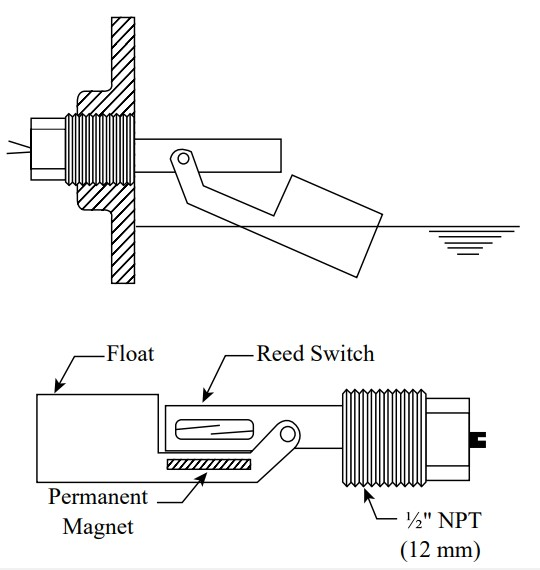
\includegraphics[width=\textwidth]{images/Screenshot_1.jpg}
        \caption{สวิตช์ลอยที่ถูกเชื่อมต่อด้วยแม่เหล็ก}
        \label{fig:mcfs1}
    \end{subfigure}
    \hfill
    \begin{subfigure}[b]{0.4\textwidth}
        \centering
        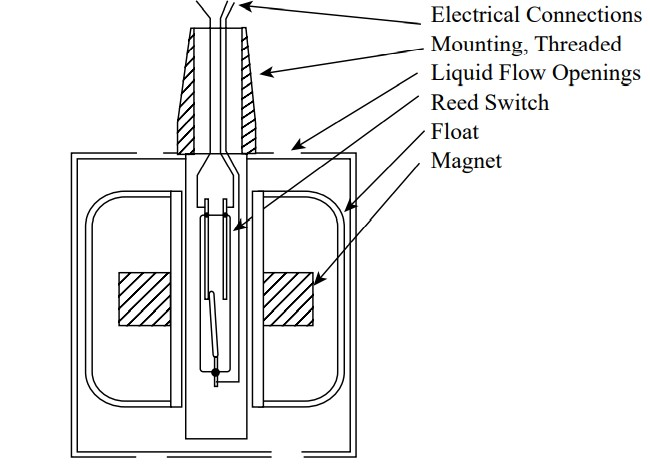
\includegraphics[width=\textwidth]{images/Screenshot_2.jpg}
        \caption{สวิตช์ลอยแบบหรีดสวิตช์}
        \label{fig:mcfs2}
    \end{subfigure}
    \hfill
    \begin{subfigure}[b]{0.4\textwidth}
        \centering
        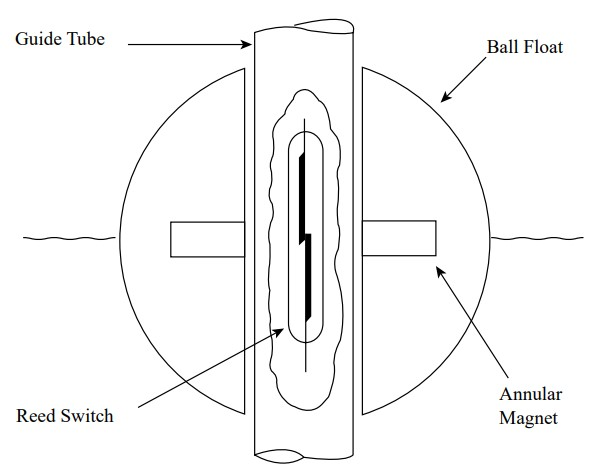
\includegraphics[width=\textwidth]{images/Screenshot_3.jpg}
        \caption{ลูกลอยและท่อนำ}
        \label{fig:mcfs3}
    \end{subfigure}
    \hfill
    \begin{subfigure}[b]{0.4\textwidth}
        \centering
        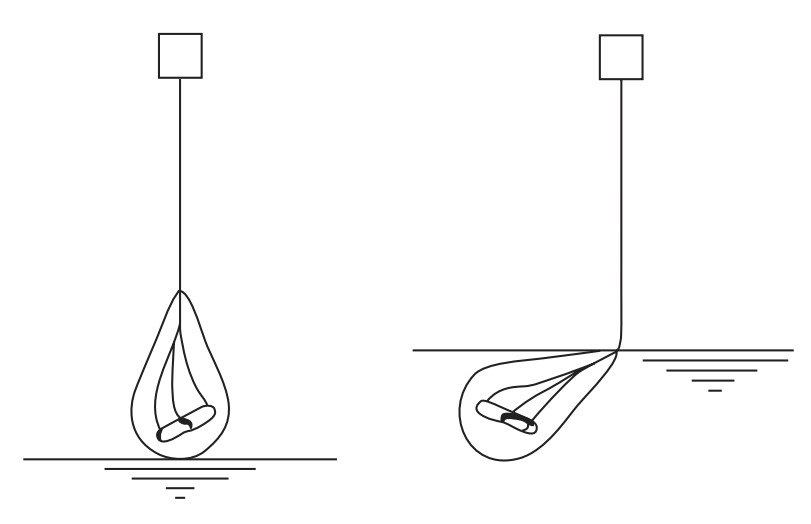
\includegraphics[width=\textwidth]{images/Screenshot_5.jpg}
        \caption{สวิตช์เอียง}
        \label{fig:mcfs4}
    \end{subfigure}
    \hfill
    \caption{โครงสร้างภายในของสวิตช์ลอยรูปแบบต่างๆ}
    \label{fig:mcfs}
\end{figure}

\subsubsection{ข้อได้เปรียบและข้อจำกัด}
เครื่องวัดระดับแบบลอยมีหลักการทำงานที่ง่าย มีโครงสร้างไม่ซับซ้อนและส่วนประกอบไม่มาก ทำให้สามารถบำรุงรักษา ซ่อมแซมได้ง่าย และเชื่อถือได้เป็นอย่างมาก
นอกจากนี้เครื่องวัดระดับแบบลอยบางรูปแบบยังสามารถทำงานภายใต้อุณหภูมิและความดันที่สูง อย่างไรก็ตาม เครื่องวัดระดับแบบลอยเป็นอุปกรณ์เฉื่อยงาน (Passive) 
ที่ไม่มีระบบตรวจสอบตนเอง จึงมีความจำเป็นต้องทำการตรวจสอบอยู่เสมอ และเนื่องจากมีการสัมผัสกับของเหลวที่จะวัดโดยตรง ของเหลวที่หนืดอาจทำให้กลไกของลูกลอยเกิดติดขัดได้

\subsection{อุปกรณ์วัดระดับทางแสง (Optical Level Device)}
อุปกรณ์วัดระดับทางแสงแบ่งตามหลักการทำงานได้เป็น 3 รูปแบบ ได้แก่การสะท้อน (Reflection), การส่งผ่าน (Transmission) และการหักเห (Refraction) 
โดยแต่ละรูปแบบก็จะมีข้อได้เปรียบและข้อจำกัดในการใช้งานที่แตกต่างกัน ในรายงานฉบับนี้จะกล่าวถึงรายละเอียดของอุปกรณ์วัดระดับทางแสงที่ใช้หลักการสะท้อน 
และการหักเหเท่าน้้น เนื่องจากอุปกรณ์วัดระดับทางแสงที่ใช้หลักการการส่งผ่าน มักใช้ตรวจจับความหนาของชั้นตะกอนของแข็งภายในของเหลว 
ซึ่งเกินขอบเขตของหัวข้อรายงานฉบับนี้

\subsubsection{หลักการทำงาน}
อุปกรณ์วัดระดับทางแสงแบบสะท้อนประกอบด้วยแหล่งกำเนิดแสง และเซนเซอร์ตรวจจับที่เป็นทรานซิสเตอร์ที่ไวต่อแสงหรือโฟโตทรานซิสเตอร์ (Phototransistor) 
บรรจุอยู่ในตัวถังเดียวกันดังภาพที่ \ref{fig:ols} (\subref{fig:ols1}) ลำแสงจากแหล่งกำเนิดแสงจะฉายไปยังของเหลวที่ทำการวัด และเมื่อระดับของของเหลวเพิ่มขึ้นจนถึงระดับหนึ่ง 
ลำแสงจะสะท้อนกลับไปยังเซนเซอร์รับแสง ทำให้โฟโตทรานซิสเตอร์นำกระแส ส่วนอุปกรณ์วัดระดับทางแสงประกอบด้วยแหล่งกำเนิดแสง 
และเซนเซอร์ตรวจจับ บรรจุอยู่ในตัวถังเดียวกันเช่นเดียวกับอุปกรณ์วัดระดับทางแสงแบบสะท้อน แต่สิ่งที่ต่างออกไปคือที่ปลายของหัววัดระดับจะถูกตัดเฉียง
เป็นมุม $45^\circ$ ดังภาพที่ \ref{fig:ols} (\subref{fig:ols2}) เมื่อเครื่องวัดถูกล้อมรอบด้วยอากาศ ลำแสงส่วนใหญ่จะสะท้อนกลับหมดภายในปริซึม ไปยังเซนเซอร์รับแสง ทำให้โฟโตทรานซิสเตอร์นำกระแส
เมื่อระดับของของเหลวที่ทำการวัดเพิ่มสูงขึ้นจนท่วมปริซึม แสงจากแหล่งกำเนิดแสงที่ตกกระทบปริซึมจะเกิดการหักเหเข้าสู่ของเหลวที่ทำการวัด เนื่องจากดัชนีหักเห
(Index of Refraction) ของของเหลวส่วนใหญ่จะมากกว่าอากาศ ทำให้โฟโตทรานซิสเตอร์หยุดนำกระแส

\begin{figure}
    \begin{subfigure}[b]{0.4\textwidth}
        \centering
        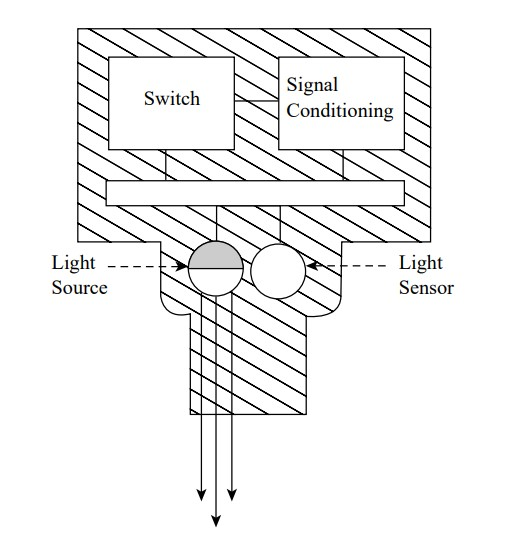
\includegraphics[width=\textwidth]{images/Screenshot_23.jpg}
        \caption{อุปกรณ์วัดระดับทางแสงแบบสะท้อน}
        \label{fig:ols1}
    \end{subfigure}
    \hfill
    \begin{subfigure}[b]{0.35\textwidth}
        \centering
        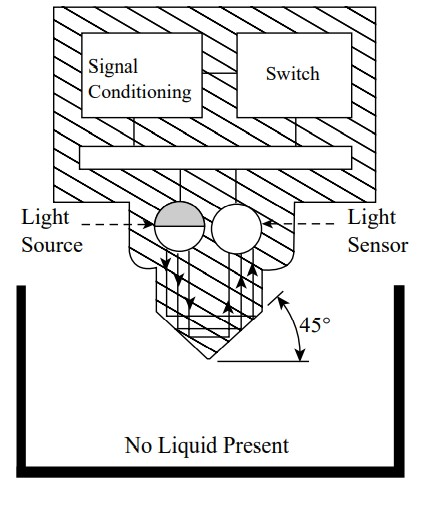
\includegraphics[width=\textwidth]{images/Screenshot_7.jpg}
        \caption{อุปกรณ์วัดระดับทางแสงแบบหักเห}
        \label{fig:ols2}
    \end{subfigure}
    \hfill
    \caption{อุปกรณ์วัดระดับทางแสงประเภทต่างๆ}
    \label{fig:ols}
\end{figure}


\subsubsection{ข้อได้เปรียบและข้อจำกัด}
อุปกรณ์วัดระดับทางแสงทั้งสองชนิดที่กล่าวมาก็มีข้อได้เปรียบและข้อจำกัดที่แตกต่างกันไป อุปกรณ์วัดระดับทางแสงแบบสะท้อนมีข้อได้เปรียบสำคัญคือ
ไม่มีการสัมผัสกับของเหลวที่ทำการวัด จึงสามารถใช้กับของเหลวที่กัดกร่อน เหนียวเหนอะหนะ และเคลือบติดได้ แต่ก็มีข้อเสียตรงที่ของเหลวที่ทำการวัดต้องทึบแสงพอสมควร
และต้องไม่มีไอ หรือความปั่นป่วนเหนือของเหลวที่ทำการวัด เพราะจะทำให้การวัดคลาดเคลื่อน ส่วนอุปกรณ์วัดระดับทางแสงแบบหักเหมีข้อดีสำคัญคือมีน้ำหนักเบา ขนาดเล็ก
และสามารถตรวจจับของเหลวปริมาณน้อยๆ ได้ แต่เนื่องจากหัววัดสัมผัสกับของเหลวโดยตรง จึงไม่สามารถใช้กับของเหลวที่กัดกร่อน เกาะติด หรือเคลือบติดได้ 
นอกจากนี้ยังอาจได้ผลบวกลวง (False Positive) หากมีหยดของของเหลวติดอยู่ที่ปลายหัววัด



\subsection{สวิตช์ระดับแบบสภาพความนำ (Conductivity-type Level Switch)}
\subsubsection{หลักการทำงาน}
สภาพความนำ (Conductivity-$\sigma$) เป็นคุณสมบัติของวัสดุ ซึ่งถูกนิยามให้เป็นความนำ (Conductance- $G$) 
หรือส่วนกลับของความต้านทาน (Resistance-$R$) ของวัสดุหนึ่ง ที่มีพื้นที่หน้าตัด $\SI{1}{cm^2}$ และยาว $\SI{1}{cm}$ 
(หน่วยของสภาพความนำคือ $\SI{}{mS.cm^{-1}}$) สำหรับของเหลวหรือสารละลาย (Solution) 
สภาพความนำเป็นฟังก์ชันของจำนวนไอออนที่มีประจุที่อยู่ในของเหลวนั้นๆ ซึ่งโดยปกติแล้วจะมีมากกว่าในอากาศ ดังนั้น 
ถ้าวงจรไฟฟ้าถูกปิดโดยสารรอบๆ ปลายหัววัดหนึ่ง กระแสที่ไหลผ่านเมื่อหัววัดนี้ถูกจุ่มลงในสารละลาย จะมากกว่ากระแสที่ไหลเมื่อหัววัดนี้ถูกล้อมรอบด้วยอากาศ
อาศัยหลักการนี้ สวิตช์สภาพความนำจึงสามารถแยกระหว่างอากาศและสารละลาย หรือระหว่างสารละลายที่นำไฟฟ้า และสารละลายที่ไม่นำไฟฟ้าได้ 

พิจารณาสวิตช์สภาพความนำดังภาพที่ \ref{fig:cls} (\subref{fig:cls1}) เมื่อรอยต่อระหว่างของเหลวและอากาศเพิ่มขึ้นสูงถึงระดับหัววัด ของเหลวจะปิดวงจรทำให้กระแสไหลจากหัววัดหนึ่ง
ไปยังอีกหัววัดหนึงได้ โดยกระแสนี้จะถูกกำหนดให้มีค่าน้อยๆ อยู่ในระดับไมโครแอมป์ เพื่อป้องกันอันตรายจากไฟฟ้าดูดและการเกิดประกายไฟ 
และความไวของสวิตช์นี้จะถูกปรับให้เข้ากับสภาพความนำของของเหลวที่ทำการวัด หัววัดทั้งสองอาจมีความยาวไม่เท่ากันดังภาพที่ \ref{fig:cls} (\subref{fig:cls2}) หรืออาจมีการหน่วงเวลา 0 ถึง 20 วินาที 
เพื่อให้มีช่วงไร้การตอบสนอง (Dead zone) หรือช่วงสมดุล (Neutral zone) ซึ่งช่วยเพิ่มความเสถียรในกรณีที่มีการกวน หรือการกระฉอกภายในถัง 

\begin{figure}
    \begin{subfigure}[b]{0.3\textwidth}
        \centering
        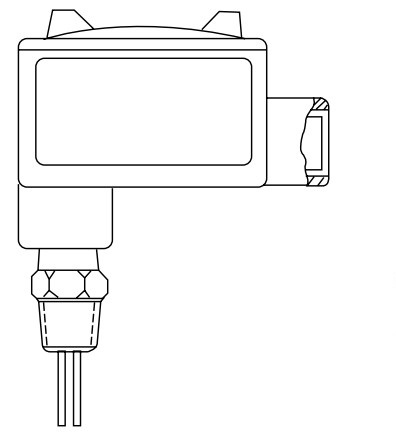
\includegraphics[width=\textwidth]{images/Screenshot_8.jpg}
        \caption{สวิตช์ระดับแบบสภาพความนำในอุตสาหกรรม}
        \label{fig:cls1}
    \end{subfigure}
    \hfill
    \begin{subfigure}[b]{0.3\textwidth}
        \centering
        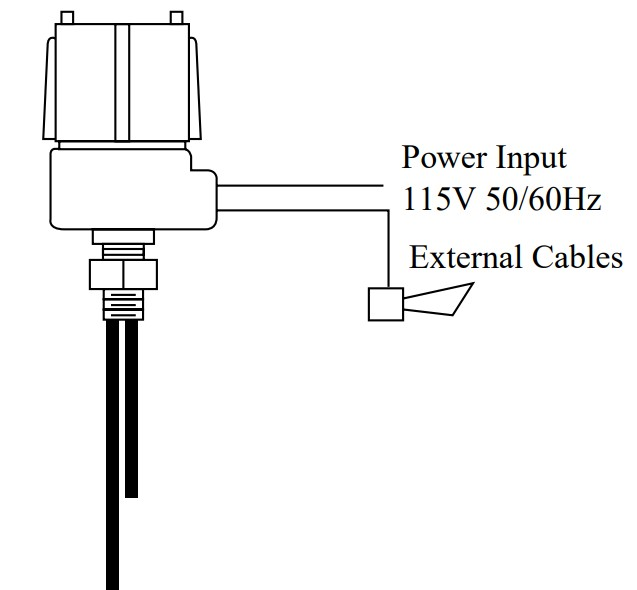
\includegraphics[width=\textwidth]{images/Screenshot_9.jpg}
        \caption{แสดงสวิตช์ระดับแบบสภาพความนำที่ถูกตัดปลายหัววัดให้ไม่เท่ากันเพื่อเพิ่มเสถียรภาพ}
        \label{fig:cls2}
    \end{subfigure}
    \hfill
    \caption{สวิตช์ระดับแบบสภาพความนำ}
    \label{fig:cls}
\end{figure}

\subsubsection{ข้อได้เปรียบและข้อจำกัด}
สวิตช์สภาพความนำมีโครงสร้างและหลักการทำงานที่ไม่ซับซ้อน ไม่มีส่วนเคลื่อนที่ที่สัมผัสกับของเหลว และสามารถนำไปใช้กับของแข็งที่ชื้นส่วนใหญ่ได้ 
ในด้านข้อจำกัด สวิตช์สภาพนำสามารถใช้ได้กับของเหลวที่นำไฟฟ้า ไม่กัดกร่อน และไม่เคลือบติดหัววัดเท่านั้น

\subsection{อุปกรณ์วัดระดับแบบความจุไฟฟ้า (Capacitance Level Device)}
\subsubsection{หลักการทำงาน} 
อุปกรณ์วัดระดับแบบความจุไฟฟ้า เป็นเครื่องวัดระดับอีกชนิด ที่สามารถวัดระดับได้ทั้งแบบต่อเนื่อง และแบบจุด 
ส่วนประกอบที่สำคัญของอุปกรณ์วัดระดับแบบความจุไฟฟ้านี้คือหัววัดหรือโพรบ ที่จุ่มลงไปในของเหลวที่ทำการวัด สัญญาณความถี่วิทยุขนาดคงตัว
ที่มีความถี่อยู่ในช่วง 0.1 - 1MHz ถูกป้อนเข้าสู่หัววัด ระดับของของเหลวหาได้จากการตรวจจับกระแสที่ไหลซึ่งเป็นสัดส่วนกับค่าแอดมิตแตนซ์ (Admittance) 
หรือค่าความจุ (Capacitance) จากแท่งยาวที่เป็นหัววัดนี้ ไปยังอิเล็กโทรดอีกอันหนึ่ง ซึ่งโดยปกติมักจะถูกเลือกให้เป็นผนังของถังเก็บ ในกรณีที่ของเหลวที่ต้องการวัด
เป็นตัวนำไฟฟ้า ($\sigma \neq 0$) หัววัดที่จะใช้จำเป็นต้องถูกเคลือบด้วยสารที่เป็นฉนวนไฟฟ้าเสียก่อนดังภาพที่ \ref{fig:cld} (\subref{fig:cld1})  กรณีนี้ไดอิเล็กตริกที่คั่นระหว่างโพรบและผนังของถังเก็บจะประกอบ
ด้วยสามส่วนคือ อากาศที่ล้อมรอบหัววัด ฉนวนที่เคลือบหัววัด และของเหลวที่ต้องการวัด แต่ถ้าหากของเหลวนั้นไม่นำไฟฟ้า เราสามารถนำหัววัดโลหะ
จุ่มลงในของเหลวได้โดยตรง (ภาพที่ \ref{fig:cld} (\subref{fig:cld1})) โดยของเหลวที่ทำการวัด และอากาศที่ล้อมรอบหัววัด จะทำหน้าที่เป็นไดอิเล็กตริก เมื่อระดับของเหลวเพิ่มขึ้น 
ค่าความจุจะเพิ่มมากขึ้น เนื่องจากค่าคงตัวไดอิเล็กตริกของตัวกลาง มีค่ามากกว่าค่าคงตัวไดอิเล็กตริกของอากาศที่ล้อมรอบ กระแสที่ไหลผ่านหัววัดก็จะเพิ่มมากขึ้นตามไปด้วย

\begin{figure}[h]
    \begin{subfigure}[b]{0.48\textwidth}
        \centering
        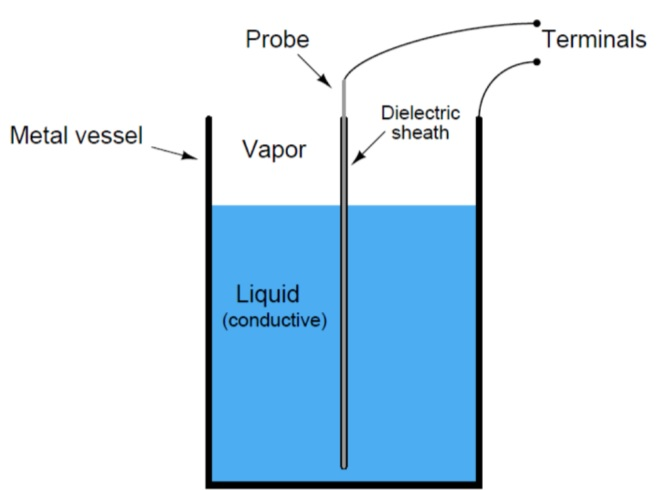
\includegraphics[width=\textwidth]{images/Screenshot_24.jpg}
        \caption{หัววัดแบบความจุไฟฟ้าในของเหลวที่เป็นตัวนำ}
        \label{fig:cld1}
    \end{subfigure}
    \hfill
    \begin{subfigure}[b]{0.48\textwidth}
        \centering
        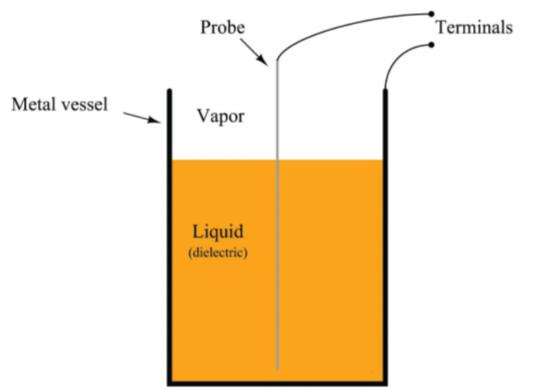
\includegraphics[width=\textwidth]{images/Screenshot_25.jpg}
        \caption{หัววัดแบบความจุไฟฟ้าในของเหลวที่เป็นฉนวน}
        \label{fig:cld2}
    \end{subfigure}
    \hfill
    \caption{หัววัดของเครื่องวัดระดับแบบความจุไฟฟ้าในของเหลวประเภทต่างๆ}
    \label{fig:cld}
\end{figure}

\subsubsection{ข้อได้เปรียบและข้อจำกัด}
อุปกรณ์วัดระดับแบบความจุไฟฟ้ามีโครงสร้างที่ง่าย มีราคาค่อนข้างถูกเมื่อเทียบกับเครื่องวัดระดับในอุตสาหกรรมประเภทอื่นๆ ไม่มีส่วนเคลื่อนที่ และทนต่อการกัดกร่อน
แต่ก็อาจเกิดความคลาดเคลื่อนได้จากหลายแหล่งไม่ว่าจะเป็นค่าคงตัวไดอิเล็กตริกของของเหลว รูปทรงทางเรขาคณิตของถังเก็บ และการเคลือบของของเหลวที่นำไฟฟ้าบนหัววัด
\subsection{สวิตช์ระดับแบบสั่นสะเทือน (Vibrating Level Switch)}
\begin{figure}[h]
    \centering
    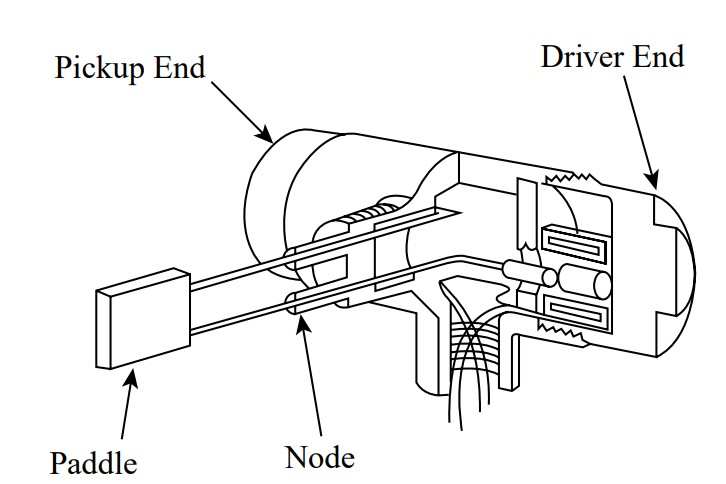
\includegraphics[width=0.4\textwidth]{images/Screenshot_11.jpg}
    \caption{โครงสร้างภายในอย่างง่ายของสวิตช์ระดับแบบสั่นสะเทือน}
    \label{fig:vls}
\end{figure}
\subsubsection{หลักการทำงาน}
สวิตช์ระดับแบบสั่นสะเทือนประกอบด้วยแหล่งกำเนิดความถี่เปียโซอิเล็กตริก (Piezoelectric Oscillator) ต่อกับหัววัดที่มีลักษณะเป็นแผ่นคล้ายใบมีด 
และตัวตรวจจับสัญญาณ ดังภาพที่ \ref{fig:vls} โดยสัญญาณป้อนกลับที่ได้รับจากตัวตรวจจับจะถูกขยาย และนำไปขับผลึกเปียโซอิเล็กตริกที่ใช้กำเนิดสัญญาณอีกครั้ง
ในสภาวะปกติ หัววัดระดับนี้จะสั่นสะเทือนด้วยความถี่ธรรมชาติหนึ่ง แต่เมื่อระดับของวัสดุ (ของเหลวหรือของแข็งที่ทำการวัด) เพิ่มขึ้นจนสัมผัสกับหัววัด 
การสั่นของหัววัดจะถูกหน่วง (Damped) ทำให้ขนาดและความถี่ของการสั่นสะเทือนลดลง ตัวตรวจจับจึงสั่งการให้รีเลย์ทำการเปลี่ยนสถานะไป

\subsubsection{ข้อได้เปรียบและข้อจำกัด}
การวัดของสวิตช์ระดับแบบสั่นสะเทือนแทบไม่ได้รับผลกระทบจากการไหล (Flow), ความปั่นป่วน (Turbulence), ฟอง (Foam), การสั่น (Vibration)
การเคลือบ (Coating) และการเปลี่ยนแปลงคุณลักษณะของวัสดุ ทำให้เป็นเทคโนโลยีการวัดระดับที่เชื่อถือได้ และสามารถใช้กับวัสดุได้หลากหลาย ไม่ว่าจะเป็นของเหลวชนิดต่างๆ,
ผงพลาสติค, นมผง, น้ำตาล, ข้าว, ธัญพืช, ฯลฯ นอกจากนี้ยังไม่ต้องการการปรับเทียบ (Calibration) และมีความสามารถตรวจสอบการทำงานของตนเอง อุปกรณ์สมัยใหม่ที่ใช้ในอุตสาหกรรม 
สามารถตรวสอบและรายงานสถานะ และความผิดปกติต่างๆ ทั้งทางไฟฟ้าและทางกลได้อย่างสม่ำเสมอ อย่างไรก็ตาม 
สวิตช์ระดับแบบสั่นสะเทือนไม่สามารถใช้กับวัสดุที่มีความหนืดมากๆ เนื่องจากวัสดุอาจจับตัวระหว่างหัววัดทั้งสอง ทำให้เกิดความผิดพลาดได้หากไม่ได้รับการตรวจสอบอย่างสม่ำเสมอ 

\subsection{อุปกรณ์วัดระดับระดับแบบอัลตราโซนิค (Ultrasonic Level Detector)}
หลักการการวัดระดับด้วยคลื่นเหนือเสียงหรืออัลตราโซนิคที่มีความถี่ระหว่าง 10 - 70 kHz สามารถนำมาสร้างเป็นเครื่องมือวัดระดับทั้งแบบจุด 
และแบบต่อเนื่องได้หลากหลายรูปแบบ โดยในรายงานฉบับนี้จะอธิบายแต่เพียงรูปแบบที่สำคัญเท่านั้น
\subsubsection{หลักการทำงาน}
เครื่องวัดระดับอัลตราโซนิคแบบจุดสามารถแยกได้เป็นสองประเภทใหญ่ๆ คือแบบหน่วงการสั่นสะเทือน (Damped Vibration Type)
และแบบดูดกลืน (Absorption Type) โดยแบบหน่วงการสั่นสะเทือน (รูปที่ \ref{fig:uld} (\subref{fig:uld1})) มีจะหลักการคล้ายกับสวิตช์ระดับแบบสั่นสะเทือน 
กล่าวคือหัววัดจะสั่นสะเทือนด้วยความถี่ธรรมชาติหนึ่ง เมื่อระดับของเหลวเพิ่มขึ้นจนถึงหัววัด ความถี่การสั่นสะเทือนจะถูกหน่วง ทำให้สถานะทางไฟฟ้าของสวิตช์เปลี่ยนไป 
ส่วนแบบดูดกลืนจะประกอบด้วยตัวส่ง (Transmitter) และตัวรับ (Reciever) จะส่งพัลส์ของคลื่นอัลตราโซนิคไปยังตัวรับผ่านของเหลวที่ต้องการวัด 
ที่ติดตั้งในรูปแบบต่างๆ (รูปที่ \ref{fig:uld} (\subref{fig:uld2})) เมื่อระดับของเหลวเพิ่มขึ้นจนท่วมหัววัด พัลส์คลื่นอัลตราโซนิคจะถูกดูดกลืน ทำให้ตัวรับตรวจจับคลื่นได้น้อยลง 
ส่วนเครื่องวัดระดับอัลตราโซนิคแบบต่อเนื่อง วัดเวลาที่คลื่นอัลตราโซนิคใช้ในการเดินทางจากตัวส่งที่เป็นลำโพงแบบอัลตราโซนิค (Ultrasonic Speaker)
ไปยังพื้นผิวของวัสดุที่ถูกวัด และสะท้อนกลับมายังตัวรับจานโลหะที่กำทอนทั้งทางไฟฟ้าและทางกล เครื่องวัดชนิดนี้สามารถติดตั้งได้หลายรูปแบบดังภาพที่ \ref{fig:ulc} ซึ่ง
เวลาสะท้อนคลื่นอัลตราโซนิคของเครื่องวัด C และ D จะเป็นตัวบอกระดับที่แท้จริง แต่สำหรับเครื่องวัด A และ B 
เวลาสะท้อนต้องถูกนำไปคำนวณโดยพิจารณาความสูงที่ติดตั้งเครื่องวัดเสียก่อน จึงจะทราบระดับได้

\begin{figure}[h]
    \begin{subfigure}[b]{0.5\textwidth}
        \centering
        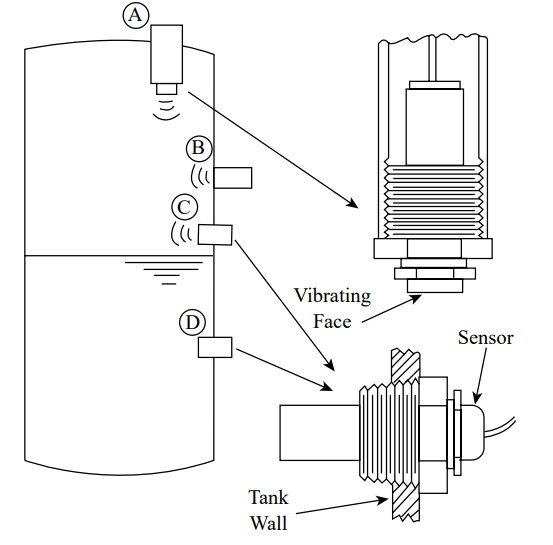
\includegraphics[width=\textwidth]{images/Screenshot_16.jpg}
        \caption{สวิตช์ระดับอัลตราโซนิคแบบสั่นสะเทือน}
        \label{fig:uld1}
    \end{subfigure}
    \hfill
    \begin{subfigure}[b]{0.5\textwidth}
        \centering
        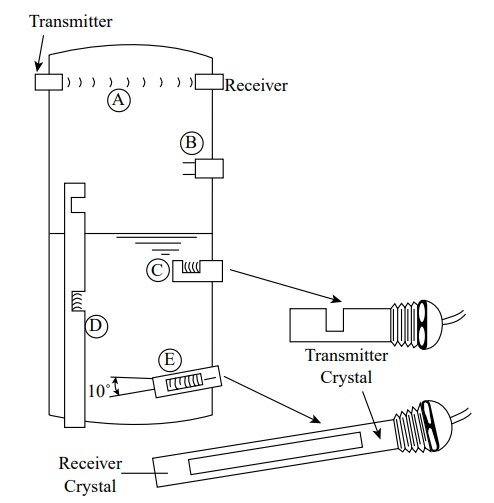
\includegraphics[width=\textwidth]{images/Screenshot_17.jpg}
        \caption{สวิตช์ระดับอัลตราโซนิคแบบดูดกลืน}
        \label{fig:uld2}
    \end{subfigure}
    \hfill
    \caption{โครงสร้าง และการติดตั้งเครื่องวัดระดับอัลตราโซนิคแบบจุดประเภทต่างๆ}
    \label{fig:uld}
\end{figure}
\begin{figure}[H]
    \centering
    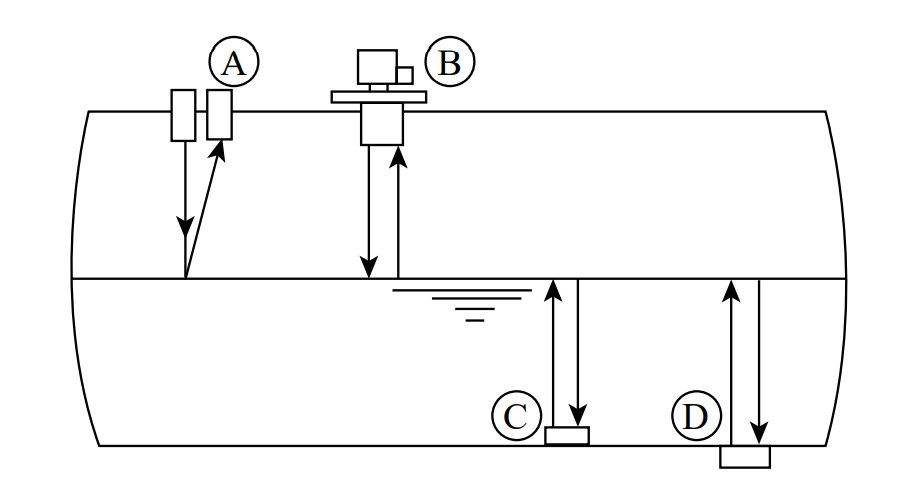
\includegraphics[width=0.5\textwidth]{images/Screenshot_26.jpg}
    \caption{ตัววัดระดับอัลตราโซนิคแบบต่อเนื่องประเภทต่างๆ}
    \label{fig:ulc}
\end{figure}

\subsubsection{ข้อได้เปรียบและข้อจำกัด}
อุปกรณ์วัดระดับระดับอัลตราโซนิคแบบจุดไม่มีส่วนเคลื่อนที่ สามารถออกแบบให้ทำการวัดโดยไม่สัมผัสได้ และบางชนิดสามารถทำการวัดได้โดยไม่ต้องเจาะทะลุถ้ง 
ทำให้สามารถวัดระดับของเหลวทีเคลือบติด และเหนียวหนืดได้ นอกจากนี้ความแม่นยำของการวัด จะไม่ขึ้นกับคุณสมบัติต่างๆ 
ของของเหลวหรือวัสดุที่ทำการวัดเช่นส่วนประกอบ ความหนาแน่น สภาพความนำไฟฟ้า และค่าคงตัวไดอิเล็กตริก
สำหรับอุปกรณ์วัดระดับระดับอัลตราโซนิคแบบต่อเนื่อง การมีตัวชดเชยทางอุณหภูมิ (Temperature Comprensator) และระบบปรับเทียบด้วยตนเอง 
(Automated Self-calibrator) เป็นสิ่งจำเป็น เนื่องจากความเร็วของคลื่นอัลตราโซนิคจะขึ้นกับอุณหภูมิ นอกจากนี้ปัจจัยต่างๆ ที่ลดทอนคลื่นสัญญาณสะท้อนกลับ
เช่น ความสูงของถัง ไอน้ำ และฝุ่นที่อยู่เหนือพื้นผิว รวมทั้งคุณสมบัติการสะท้อน และความหนาแน่นของพื้นผิวของวัสดุที่ทำการวัด ก็ส่งผลต่อความแม่นยำของการวัดเช่นกัน

\subsection{อุปกรณ์วัดระดับแบบเรดาร์ (Radar Level Transmitter)}
อุปกรณ์วัดระดับแบบเรดาร์ใช้คลื่นแม่เหล็กไฟฟ้า ซึ่งโดยปกติคือคลื่นไมโครเวฟในย่าน K และ X ($\approx 6$ ถึง $\SI{28}{GHz}$) 
เพื่อทำการวัดระดับของเหลวอย่างต่อเนื่อง อุปกรณ์วัดระดับแบบเรดาร์สามารถแบ่งได้เป็นสองประเภทหลักๆ คือ อุปกรณ์วัดระดับเรดาร์แบบไม่สัมผัส
(Non-Contacting Radar Level Transmittor) และ เครื่องวัดระดับเรดาร์แบบบังคับนำคลื่น (Guided Wave Radar Level Transmittor) 
\subsubsection{หลักการทำงาน} 
อุปกรณ์วัดระดับเรดาร์แบบไม่สัมผัสมักใช้หลักการ FMCW (Frequency Modulated Continuous Wave) ในการวัด 
โดยตัวส่งสัญญาณจะทำการกวาดความถี่ (Frequency Sweep) หรือกำเนิดสัญญาณความถี่เพิ่มขึ้นเรื่อยๆ อย่างเชิงเส้น ภายใต้แบนวิตธ์ และเวลาการกวาด
(Sweep Time) ที่คงตัว ดังภาพที่ \ref{fig:rtl} (\subref{fig:rtl1}) คลื่นจากตัวกำเนิดจะสะท้อนกับพื้นผิวของของเหลว กลับมายังตัวตรวจจับที่ตรวจจับความถี่ที่ส่งออก และสะท้อนกลับมาพร้อมๆ กัน
ผลต่างของความถี่ที่ส่งไปใหม่ และสะท้อนกลับมา จะเป็นสัดส่วนโดยตรงกับระยะเวลาที่คลื่นใช้ในการเดินทาง (Time of Flight) 
และระยะห่างระหว่างเครื่องวัดกับพื้นผิวของของเหลว การใช้เทคนิคมอดุเลทความถี่มีข้อได้เปรียบที่สำคัญคือ สัญญาณรบกวนภายในถังเก็บที่อยู่ในโดเมนขนาด 
(Amplitude Domain) จะไม่มีผลต่อความแม่นยำของการวัด ส่วนอุปกรณ์วัดระดับเรดาร์แบบบังคับนำคลื่นจะทำการวัดระดับด้วยกระบวนการ TDR 
(Time Domain Reflectrometry) คือทำการปล่อยคลื่นแม่เหล็กไฟฟ้าความถี่สูงแต่มีขนาดต่ำ ผ่านสายส่ง (Transmission Line), เคเบิล (Cable) 
หรือตัวบังคับนำคลื่น (Waveguide) แลัวตรวจจับขนาดของสัญญาณที่สะท้อนกลับมาเป็นระยะๆ ระยะเวลาระหว่างสัญญาณที่ส่งออกไป 
และสะท้อนกลับมาจะสามารถนำมาหาตำแหน่งที่อิมพีแดนซ์ของโพรบวัดนี้ไม่ต่อเนื่อง (จุดที่ของเหลวท่วมหัววัดอยู่) ได้ (ภาพที่ \ref{fig:cld} (\subref{fig:rtl2}))

\begin{figure}
    \begin{subfigure}[b]{0.4\textwidth}
        \centering
        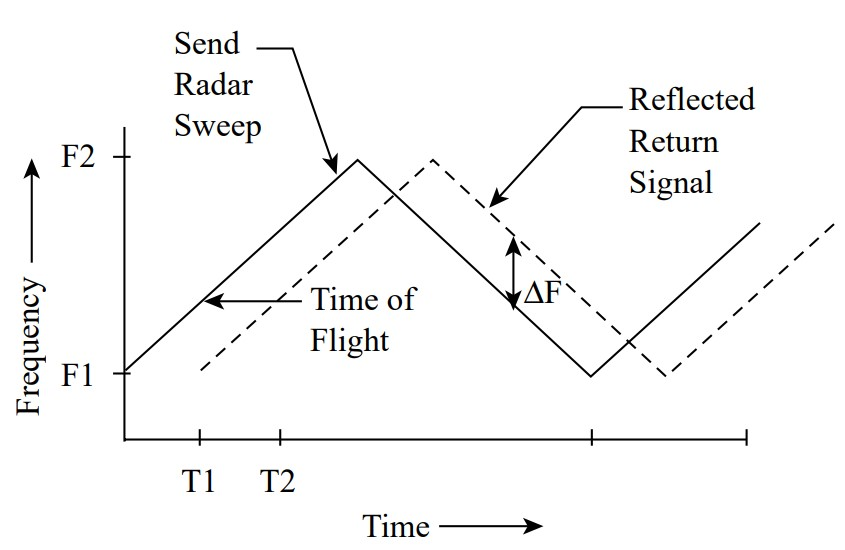
\includegraphics[width=\textwidth]{images/Screenshot_19.jpg}
        \caption{การวัดระดับด้วยเทคนิค FMCW: ผลต่าง $\Delta F$ ของความถี่จะเป็นสัดส่วนกับระดับของเหลว}
        \label{fig:rtl1}
    \end{subfigure}
    \hfill
    \begin{subfigure}[b]{0.6\textwidth}
        \centering
        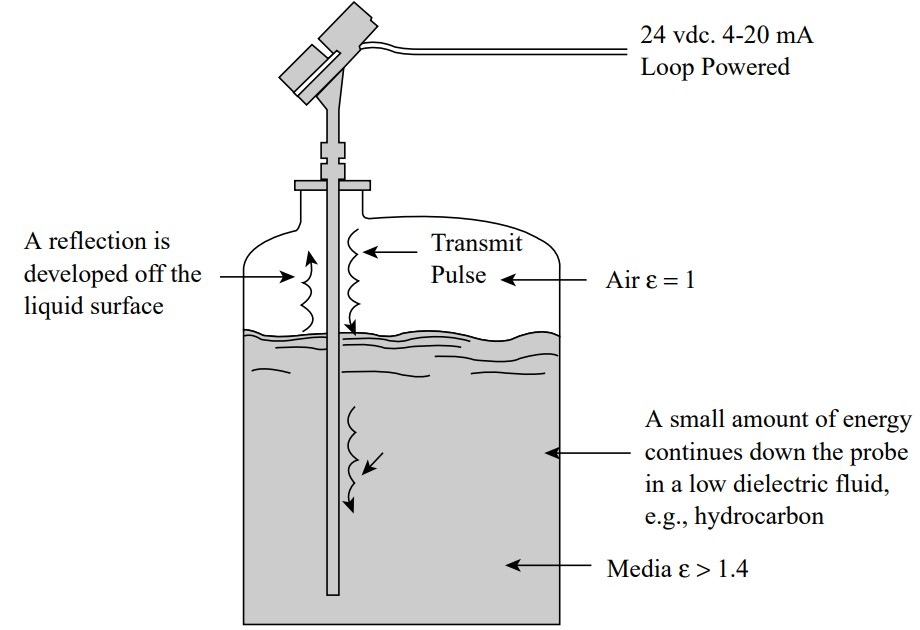
\includegraphics[width=\textwidth]{images/Screenshot_18.jpg}
        \caption{การวัดระดับด้วยเทคนิค TDR}
        \label{fig:rtl2}
    \end{subfigure}
    \hfill
    \caption{การวัดระดับของเครื่องวัดระดับแบบเรดาร์ด้วยเทคนิค FMCW และ TDR}
    \label{fig:rtl}
\end{figure}

\subsubsection{ข้อได้เปรียบและข้อจำกัด}
อุปกรณ์วัดระดับแบบเรดาร์เป็นเครื่องวัดที่มีประสิทธิภาพค่อนข้างมาก สามารถใช้กับวัสดุที่ต้องการวัดได้หลากหลาย และมีจุดเด่นสำคัญที่เหนือกว่าอุปกรณ์วัดระดับแบบอัลตราโซนิคคือ
อัตราเร็วของคลื่นเรดาร์เปลี่ยนแปลงในตัวกลาง และอุณหภูมิต่างๆ น้อยกว่าอัตราเร็วของคลื่นอัลตราโซนิคมาก แต่อย่างไรก็ตาม 
อุปกรณ์วัดระดับแบบเรดาร์มีข้อจำกัดคือไม่สามารถใช้ได้เมื่อวัสดุที่ต้องการวัดระดับเป็นฉนวนที่มีค่าคงตัวไดอิเล็กตริกน้อยกว่า 1.4 ($\epsilon < 1.4$) 
เนื่องจากจะทำให้สัญญาณที่สะท้อนกลับมามีขนาดที่น้อยจนตรวจจับไม่ได้

เครื่องวัดระดับเรดาร์แบบไม่สัมผัสมีข้อเด่นคือไม่สัมผัสกับวัสดุที่ทำการวัด แต่ก็ถูกรบกวนโดยการคน 
ฟอง และการรบกวนจากแหล่งอื่นๆ ได้ง่ายกว่าเครื่องวัดระดับแบบบังคับนำคลื่น ที่ต้องมีหัววัดสัมผัสจุ่มลงไปในของเหลว นอกจากนี้ความแม่นยำของการวัดระดับด้วยกระบวนการ
FMCW ขึ้นกับความเที่ยงตรงของตัวกำเนิดความถี่ซึ่งสัมพันธ์กับราคาของเครื่องวัด ทำให้เครื่องวัดระดับเรดาร์แบบไม่สัมผัสที่เที่ยงตรงสูงมีราคาแพงมาก
\newpage
\section{บทสรุป}
การวัดระดับในอุตสาหกรรมเมื่อมองเผินๆ อาจดูเหมือนว่าเป็นเรื่องไกลตัว แต่ถ้าหากพิจารณาสิ่งต่างๆ รอบๆ ตัวเราอย่างละเอียด ก็จะพบได้ว่าการวัดระดับนั้น 
แท้ที่จริงแล้วเป็นฟันเฟืองที่สำคัญหนึ่งที่ขับเคลื่อนโลกยุคปัจจุบัน น้ำหวานในร้านสะดวกซื้อ กระดาษที่วางอยู่บนโต๊ะ
รวมไปถึงแชมพู สบู่เหลวในห้องน้ำและน้ำยาล้างจานในห้องครัวที่ไม่อาจแยกออกจากวิถีชีวิตของมนุษย์ ล้วนผ่านกระบวนการทางอุตสาหกรรม
ที่การวัดระดับมีบทบาทสำคัญในการควบคุมจัดการกระบวนการผลิตทั้งสิ้น การจัดทำรายงานฉบับนี้นอกจากกลุ่มผู้จัดทำจะได้ศึกษา 
และค้นคว้าวิธี และหลักการวัดระดับในอุตสาหกรรมจากแหล่งต่างๆ แล้ว ยังทำให้ได้ตระหนักถึงความสำคัญของการวัดและเครื่องมือวัด ที่มีผลต่อการพัฒนาทางอุตสาหกรรม
และคุณภาพชีวิตของมนุษย์อีกด้วย อีกสิ่งหนึ่งที่น่าทึ่งคือศาสตร์แห่งการวัดระดับนั้นเป็นการผสานเอาองค์ความรู้ต่างๆ เช่นคาน การสะท้อนและหักเหของแสง วงจรไฟฟ้า 
การสะท้อนของเสียง และการประมวลสัญญาณ เพื่อสร้างเครื่องวัดระดับที่เหมาะสมสอดคล้องกับของเหลว และสภาพการผลิตในอุตสาหกรรมที่หลากหลาย 
ซึ่งบางชนิดก็มีหลักการทำงานที่มีซับซ้อน แต่ขณะเดียวกันก็น่าสนใจอย่างน่าเหลือเชื่อ ในที่สุดแล้ว 
ไม่มีเครื่องวัดระดับ หรือหลักการวัดระดับใดในโลกที่ดีที่สุดเสมอ มีเพียงแต่เครื่องวัดระดับต่างๆ ที่เหมาะกับการใช้งานในสภาพแวดล้อมนั้นๆ 
ซึ่งจะต้องถูกเลือกเหมาะสมโดยการพิจารณาเงื่อนไขต่างๆ อย่างละเอียด
\newpage
\nocite{*}
\bibliography{reportbib}
\bibliographystyle{plain}
\end{document}